\documentclass[a4paper,12pt,bibliography=totoc,index=totoc,twoside,francais]{scrbook}
%\documentclass[a4paper,12pt,DIVcalc,bibliography=totoc,index=totoc,twoside,francais]{scrbook}
\KOMAoptions{titlepage,chapterprefix,open=right}
%\KOMAoptions{bibliography=totoc,index=totoc}
%\addtokomafont{chapter}{\rmfamily}
%\addtokomafont{section}{\rmfamily}

\usepackage[utf8]{inputenc}
\usepackage[T1]{fontenc}
\usepackage{lmodern}
\usepackage{graphicx}
\usepackage[automark,headsepline]{scrpage2}
\usepackage[style=numeric,sorting=none,backend=biber]{biblatex}
\usepackage{csquotes}
\usepackage{xspace}
\usepackage[autolanguage]{numprint}
\usepackage{array}
\usepackage{booktabs}
\usepackage[table,svgnames,dvipsnames]{xcolor}
\usepackage[final]{pdfpages} 
\clubpenalty=5000
\widowpenalty=5000

\usepackage{graphicx,wrapfig}

%\usepackage{lipsum}
%\bibliography{biblio}

\usepackage[backend=biber]{biblatex}
\addbibresource{biblio.bib}

%\usepackage{hyperref} 
\usepackage[pdfauthor={Cynthia Lopes do Sacramento}, pdftitle={Applications SDN}]{hyperref}

\usepackage{makeidx}
\makeindex

\setlength{\parskip}{1em}
\renewcommand{\baselinestretch}{1.2}

%\usepackage[xindy={language=french,codepage=utf8},acronym,toc=true,nonumberlist]{glossaries}
%\usepackage[acronym,toc=true,nonumberlist]{glossaries}
\usepackage[toc=true,acronym,nopostdot,nonumberlist]{glossaries}
%\usepackage[toc=true,acronym]{glossaries}

\makeglossaries


\let\Oldgls\gls%Transformation de la commande \gls en \Oldgls
\let\Oldglslink\glslink%Transformation de la commande \gls en \Oldgls
\let\Oldglspl\glspl%Transformation de la commande \gls en \Oldgls

% Création de la nouvelle commande \gls
\renewcommand{\gls}[1]{%
\textbf{\Oldgls{#1}}%
}
% Création de la nouvelle commande \gls
\renewcommand{\glslink}[2]{%
\textbf{\Oldglslink{#1}{#2}}%
}
% Création de la nouvelle commande \gls
\renewcommand{\glspl}[1]{%
\textbf{\Oldglspl{#1}}%
}

%\newacronym{rtfm}{RTFM}{Read the f\dots manual}

\newacronym{sdn}{SDN}{Software-Defined Networking : Réseau Informatique Défini par Logiciel}

\newacronym{ti}{TI}{Technologie de l'Information}

\newacronym{si}{SI}{Système d'Information}

\newacronym{nfv}{NFV}{Network Functions Virtualization, Virtualisation des fonctions réseau}

\newacronym{onf}{ONF}{Open Networking Foundation}

\newacronym{nos}{NOS}{Network Operating System, Système d'exploitation réseau}

\newacronym{vm}{VM}{Virtual Machine, Machine Virtuelle}

\newacronym{ip}{IP}{Internet Protocol, Protocole d'Internet}

\newacronym{vlan}{VLAN}{Virtual Local Area Network, Virtual LAN}

\newacronym{lan}{LAN}{Local Area Network, Réseau local}

\newacronym{wan}{WAN}{Wide Area Network, Réseau étendu}

\newacronym{nat}{NAT}{Network Address Translation, Traduction d'adresse réseau}

\newacronym{dhcp}{DHCP}{Dynamic Host Control Protocol, Protocole pour la configuration automatique d'hôte}

\newacronym{dns}{DNS}{Domain Name System, Système de noms de domaine}

\newacronym{mpls}{MPLS}{MultiProtocol Label Switching, Commutation multi-protocoles par étiquettes}

\newacronym{ids}{IDS}{Intrusion Detection System, Système de Détection d'Intrusion}

\newacronym{ips}{IPS}{Intrusion Prevention System, Système de Prévention d'Intrusion}

\newacronym{one}{ONE}{Open Network Environment, Environnement Réseau Ouvert}

\newacronym{api}{API}{Application Programming Interface, Interface de Programmation}

\newacronym{asic}{ASIC}{Application Specific Integrated Circuit, Circuit intégré pour application spécifique}

\newacronym{iaas}{IaaS}{Infrastructure as a Service, Infrastructure en tant que service}

\newacronym{http}{HTTP}{HyperText Transfer Protcol, Protocole de transfert de hypertexte}

\newacronym{qos}{QoS}{Quality of Service, Qualité de service}

\newacronym{ietf}{IETF}{Internet Engineering Task Force, Détachement d'ingénierie d'internet}

\newacronym{irtf}{IRTF}{Internet Research Task Force, Détachement de recherche d'internet}

\newacronym{aci}{ACI}{Application Centric Infrastructure, Infrastructure centrée sur les applications}

\newacronym{sds}{SDS}{Software Defined-Storage, Stockage Défini par Logiciel}


\newglossaryentry{paradigme}
{
  name=Paradigme,
  text=paradigme,
  description={Un paradigme consiste en une collection de règles, standards et exemples de pratiques scientifiques, partagés par un groupe de scientifiques. 
  Sa genèse et poursuite en tant que tradition de recherche sont conditionnées à un fort engagement et consensus des personnes impliquées. \cite{paradigmdef}
  D'après Dosi \cite{newparadigm}, quand un nouveau paradigme technologique apparaît, il représente une discontinuité ou un changement dans la manière de penser. Ce changement apporté par le paradigme est souvent lié à une sorte d'innovation radicale qui implique une nouvelle technologie. Dans ce document, le terme paradigme sera employé dans ce sens d'innovation et application de nouvelle technologie.  }
}

\newglossaryentry{scalability}
{
  name=Scalabilité,
  text=scalabilité,
  description={ Terme provenant de l'anglicisme \textit{scalability} qui exprime la capacité d'être mis à échelle. En informatique cela désigne la capacité d'un système, d'un réseau ou un processus de gérer l'augmentation ou la réduction de la charge de manière à pouvoir la gérer. \cite{scalability}. Le terme est souvent employé pour exprimer une extensibilité, évolutivité ou passage à l'échelle, mais il n'y <<a pas d'équivalent communément admis en français >>. \cite{chevance2001serveurs}  }
}

%n'a pas d'équivalent communément admis en français


\newglossaryentry{abstraction}
{
  name=Abstraction,
  text=abstraction,
  description={  En informatique, l'abstraction est un terme souvent employé pour désigner le mécanisme et la pratique qui réduisent et factorisent les détails négligeables de l'idée exprimée afin de se focaliser sur moins de concepts à la fois.
     C'est aussi la notion de couches d'abstraction utilisée comme moyen pour gérer la complexité des systèmes informatiques où les couches correspondent à des niveaux de détails appliqués. \cite{AbstractionCS}
  }
}


%Scalability is the ability of a system, network, or process to handle a growing amount of work in a capable manner or its ability to be enlarged to accommodate that growth.

\newglossaryentry{bigdata}
{
  name=Big Data,
  description={Big Data est un terme appliqué aux ensembles de données dont la taille (ou le format) est au-delà de la capacité des outils logiciels communs, qui ne peuvent plus les capturer, les gérer et les traiter. Une nouvelle classe de technologies et outils a été développée pour attribuer une valeur commerciale à ces données grâce à une analyse complexe. Le terme est employé en  référence à ce type de données ainsi qu'aux technologies utilisées pour les stocker et les traiter.
  \cite{IMBigData}    }
}


\newglossaryentry{cluster}
{
  name=Cluster,
  text=cluster,
  description={  En réseaux informatiques, un cluster désigne un groupe des machines reliées entre elles à l'aide d'un réseau de communication. Cette configuration est souvent utilisée pour réaliser des calculs à haute performance. \cite{cluster} }
}


\newglossaryentry{cloudcomputing}
{
  name=Cloud Computing,
  text=cloud computing,
  description={  Cloud Computing, ou informatique dans les nuages, est une évolution de la fourniture de services \gls{ti} qui offre un moyen d'optimiser l'usage et le déploiement rapide de ressources. Cela se fait par des systèmes et solutions plus efficaces et \glslink{scalability}{scalables}, fournissant un niveau plus haut d'automatisation. Diverses entreprises ont adopté le cloud computing et réalisent des avantages significatifs en agilité, réduction de coûts et soutien de la croissance du business. \cite{CloudComputingIntelVisionSpeeding}      }
}



\newglossaryentry{virtualisation}
{
  name=Virtualisation,
  text=virtualisation,
  description={  Pour diverses entreprises, l'infrastructure serveur virtualisée est la base sur laquelle le \glslink{cloudcomputing}{cloud} est construit. Initialement, les technologies de virtualisation ont permis aux data centers de consolider leurs infrastructures pour réduire les coûts. Avec le temps, l'intégration des technologies pour le management flexible de ressources a facilité une allocation plus dynamique. Cela a aidé à réduire les coûts et a également augmenté la flexibilité et la performance. \cite{CloudComputingIntelVisionSpeeding}  }
}



\newglossaryentry{datacenter}
{
  name=Data  Center,
  text=data center,
  description={  Centre de traitement de données. Il s'agit d'une installation utilisée pour héberger des systèmes informatiques et les composants associés, comme les systèmes de télécommunication et de stockage. En général, un data center inclut alimentation et  connexions des données redondantes, contrôles d'environnements comme la climatisation ainsi que divers dispositifs de sécurité. \cite{dataCenterDef} }
}
\newglossaryentry{middlebox}
{
  name=Middlebox,
  text=middlebox,
  description={  Boîtier intermédiaire. Un middlebox est un serveur conservant des états de la communication entre deux hôtes. Ils se différencient des hôtes qui représentent les extrémités de la communication. Ils sont encore différents des routeurs qui ne gardent pas d'états concernant les sessions de communications.  \cite{InternetEvolutionRoleSoftwareEngineeringRealInternet}  },
  plural=middleboxes
}

\newglossaryentry{openflow}
{
  name=OpenFlow,
  description={   Le protocole OpenFlow vise à standardiser l'interface entre les applications et le contrôleur  ainsi que l'interface entre le contrôleur et les éléments de commutation. \cite{SurveySDNArchi} \cite{OpenFlowStanfordSwitch}  }
}


\newglossaryentry{controlplane}
{
  name=Plan de Contrôle,
  text=plan de contrôle,
  description={  Intelligence du réseau, ensemble des données locales utilisées pour établir les entrées des tableaux de commutation, qui sont utilisés par le plan de données pour effectuer la transmission du trafic entre les ports d'entrée et de sortie du dispositif. \cite{sdnbookControlDataPlanes} },
  plural={Plans de contrôles}
}

\newglossaryentry{dataplane}
{
  name=Plan de Données,
  text=plan de données,
  description={  Le plan de donnés traite les data-grammes entrants dans le média à travers une série d'opérations au niveau des liens qui collectent ces data-grammes et réalisent divers tests de cohérence basiques. Ensuite les data-grammes sont transférés en accord avec des tableaux pré-remplis par le \gls{controlplane}.  \cite{sdnbookControlDataPlanes}},
  plural={plans de données}
}

\newglossaryentry{opensource}
{
  name=Open Source,
  text=open source,
  description={ Logiciel avec code source ouvert, qui peut donc être utilisé librement, modifié et partagé par quelqu'un. Un logiciel open source est développé par plusieurs personnes et distribué sous des licences qui se conforment à la définition d'open source.  \cite{OpenSource}  }
}

\newglossaryentry{opendaylight}
{
  name=Open Daylight,
  description={ Association initiée par Linux Foundation pour l'union des géants du marché réseau dans le but de développer un contrôleur SDN open source, pour l'innover, l'encourager et pour permettre son adoption accélérée. \cite{OpenDaylight} }
}


\newglossaryentry{fabric}
{
  name=Fabric,
  text=fabric,
  description={ En informatique, fabric (qui signifie tissu en anglais) est un synonyme de plate-forme ou structure.  En général, le terme fabric décrit la façon dont différents composants travaillent ensemble pour former une entité unique. Dans ces systèmes la liaison entre les composants est tellement dense qu'un schéma représentant leurs relations rassemblerait à une pièce de tissu tricotée.
  Sous ce terme généralement admis par l'industrie réseau, un fabric est une topologie réseau dans laquelle les composants transmettent des données l'un à l'autre  à travers les switches d’interconnexion.
  % En théorie, un \textit{fabric} devrait être capable de supporter un grand nombre de conceptions de pointe y compris des schémas d'adressage et des modèles de politique. 
  \cite{NetworkFabricSearchSDN} \cite{fabricExtending}}
}

\usepackage[english,francais]{babel}
\frenchbsetup{og=«, fg=»}



\pagestyle{scrheadings}

\begin{document}
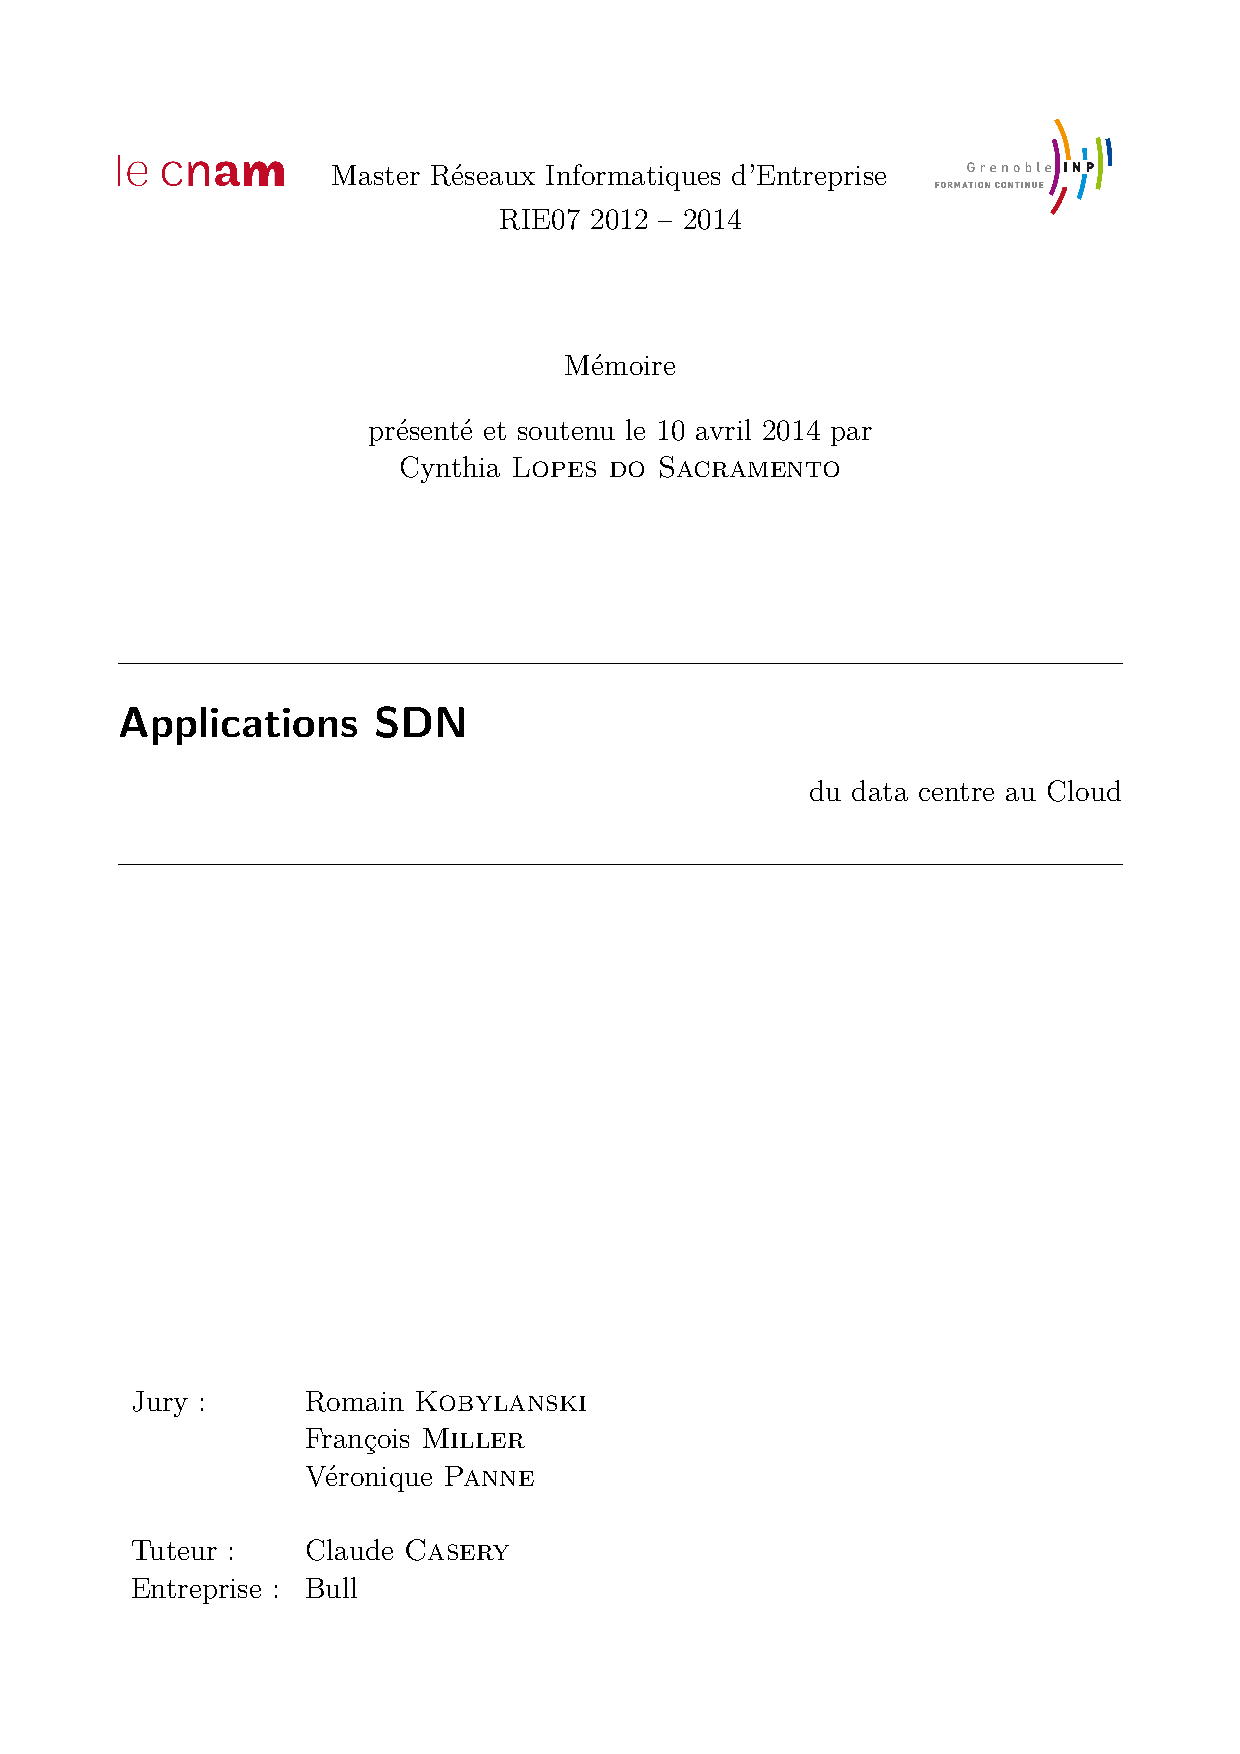
\includepdf[pages={1-2}]{couverture-ebt.pdf}

\frontmatter
%\begin{flushright}
%It is a sad age when it is more difficult to break a prejudice than an atom.\\
%Albert \bsc{Einstein}\\
%\end{flushright}

\tableofcontents
\listoftables
\listoffigures

\mainmatter
%\addchap{Introduction}
\addchap{Introduction}

%Most IT infrastructures were not built to support the explosive growth in computing capacity and information that we see today. Many data centers have become highly distributed and somewhat fragmented. As a result, they are limited in their ability to change quickly and support the integration of new types of technologies or to easily scale to power the business as needed.

%When equipped with a highly efficient, shared, and dynamic infrastructure, along with the tools needed to free up resources from traditional operational demands, IT can more efficiently respond to new business needs. As a result, organizations can focus on innovation and on aligning resources to broader strategic priorities. Decisions can be based on real-time information.

Les centres de traitement de données évoluent aujourd'hui à un rythme intense pour accompagner l'explosion constatée dans l'utilisation (en volume et en diversité) de données. L'accélération de l'innovation\index{Innovation} dans l'informatique impose une rénovation constante des infrastructures des entreprises. La virtualisation\index{Virtualisation} a permis aux centres de données d'améliorer la productivité de leurs serveurs, mais pour arriver à l'agilité\index{Agilité} souhaitée, les data centres doivent faire évoluer leurs réseaux. % pour pouvoir passer au Cloud Computing. 
Cette étude analyse les applications \gls{sdn}\index{SDN} pour distinguer quels sont les apports dans le contexte actuel et futur des data centres et habiliter le passage au \gls{cloudcomputing}.\index{Cloud Computing}

\par 
La plupart des infrastructures de \gls{ti} n'ont pas été construites pour supporter la croissance explosive des données constatée aujourd'hui et n'ont pas la capacité de traitement de l'information\index{Compute} demandée. Plusieurs centres de traitement de données sont devenus hautement distribués et relativement fragmentés par rapport aux besoins des différents profils des clients. Ils se trouvent donc limités dans leur capacité à évoluer rapidement et à supporter l'intégration des nouveaux types de technologies ou à se mettre à l'échelle des besoins de ses utilisateurs.

\par 
Lorsqu'ils sont équipés d'infrastructures performantes, partagées et dynamiques ainsi que des outils nécessaires pour adapter les ressources\index{Ressources} à la demande, les \gls{si} peuvent répondre efficacement aux besoins métiers. Ainsi, les structures pourraient se focaliser sur l'innovation\index{Innovation} et l'adaptation des ressources selon les priorités stratégiques de leurs métiers. Cela faciliterait la prise de décisions, qui pourrait être concentrée sur l'information en temps-réel. \cite{hpAlcatelCreatinCloudDCchallenges}

\par
Alors que le coût du réseau dans un data centre est estimé à 15\% du total, sans être un des plus élevés, il est largement établi qu'il représente un élément clé pour la réduction des coûts\index{Coûts} et l'augmentation du retour sur investissement. Les coûts d'investissement dans les serveurs ont été évalués à 45\% des coûts des data centres. Malheureusement la charge\index{Charge} utile des serveurs est remarquablement basse, arrivant à seulement 10\% d'utilisation dans certains exemples.  \cite{cloudCosts}

\par 
La technique de la virtualisation\index{Virtualisation} a permis le partage des processus entre machines, mais des contraintes réseau continuent à limiter l'agilité\index{Agilité} dans les data centres. L'agilité est définie par la capacité de placer tout service n'importe où dans le data centre, tout en assurant la sécurité\index{Sécurité}, la performance et l'isolation entre tous les services. Les designs des réseaux conventionnels dans un data centre empêchent cette agilité ; par nature ils fragmentent  à la fois les réseaux et la capacité des serveurs, limitant et réduisant la croissance dynamique des pools de serveur et de traitement de l'information\index{Compute}. \cite{cloudCostsAgility}



\par 
L'agilité est donc un élément clé ; certaines entreprises s'évertuent à déployer de nouvelles applications ou faire évoluer les existantes au rythme de la croissance de leur business. Selon le sondage mené par AlgoSec avec 240 professionnels de l'informatique, 25\% des organisations participantes doivent attendre plus de 11 semaines pour qu'une nouvelle application soit mise en ligne (et dans 14\%, ce temps dépasse 5 mois). Les résultats révèlent également que 59\% des entreprises ont besoin de plus de huit heures pour réaliser un changement de connectivité dans une application. \cite{algoSecSurvey}


\par
Cependant, lors du passage au Cloud, les entreprises réalisent que la virtualisation\index{Virtualisation} des serveurs est considérablement limitée par les designs Ethernet classiques et les contrôles de sécurité réseau traditionnels. Avec l'augmentation de la virtualisation au sein des data centres, quatre tâches majeures deviennent critiques :
\begin{itemize}
\item Prévention de la congestion du trafic ;
\item Réduction de la complexité\index{Complexité} mise en place des politiques réseau et maintien du niveau de service;
\item Élimination des points aveugles qui conduisent à des pannes ;
\item  Scellement des failles de sécurité pour protéger les données. \cite{virtualizedCCCC}\\
\end{itemize}
%But as businesses move to the private cloud, they are finding server virtualization is severely limited by clas- sic Ethernet designs and traditional network security controls. As data center virtualization scales, four critical tasks become increasingly cumbersome:n Preventing traffic bottlenecksn Reducing complexity of network policy and service level assurancen Eliminating management blind spots that lead to outagesn Sealing up security loopholes to protect data

\par
Cette étude a pour but de démontrer comment SDN\index{SDN} peut être appliqué aux réseaux pour permettre aux data centres de passer au Cloud Computing, et dépasser les limites du réseau actuel. Dans le premier chapitre, le contexte des data centres sera défini. Ensuite, les problématiques dans l'aspect réseau seront exposées. Enfin, le dernier chapitre présentera SDN et démontrera ses apports dans ce cadre.




\chapter{Les évolutions du business modèle des Data Centres}
\label{chap-1}

Ce chapitre a pour but de définir un data centre afin de pouvoir analyser ses problématiques, enjeux et solutions possibles, en vue de comprendre son état actuel et ses limites par rapport aux nouveaux besoins et défis business. Les éléments plus importants de la conception et de l'architecture du data centre seront présentés ainsi que les difficultés qui l'ont amené faire à évoluer son modèle de livraison vers l'approche Cloud Computing.

\section{Data centres et leurs objectifs}

Un data centre (aussi nommé \og ferme de serveurs \fg{}) est un répertoire centralisé pour le stockage, management et distribution de données et informations. Typiquement, un data centre est une installation utilisée pour loger des systèmes informatiques et ses composants associés, tels que systèmes de télécommunication et stockage. 

Les data centres traditionnels hébergent historiquement de nombreuses applications relativement petites ou moyennes, chacune s'exécutant dans une infrastructure matérielle dédiée qui est isolée et protégée des autres systèmes dans la même installation. Ces data centres accueillent du matériel et du logiciel pour multiples unités organisationnelles ou même diverses entreprises. Différents systèmes informatiques au sein d'un tel data centre ont souvent très peu d'éléments en commun en termes de matériel, logiciel ou infrastructure de maintenance, et en général ne communiquent pas entre eux. 


Les tendances de l'informatique vers une approche côté serveur et l'explosion en popularité des services sur internet ont changé ce scénario. Des infrastructures data centre entières ont été dédiées à un seul acteur pour faire fonctionner ses services offerts. Dans ce cadre, un data centre appartient à une seule organisation et utilise des matériels et plateformes logicielles relativement homogènes qui partagent une couche commune de systèmes de management. Ces data centres dédiés exécutent un nombre réduit d'applications (ou services internet) beaucoup plus importants en taille; l'infrastructure commune de management permet alors une meilleure flexibilité de déploiement. 

Ces infrastructures sont montées pour gérer la taille des applications déployées et la haute disponibilité exigée pour ces services, visant en général 99,99\% de durée de fonctionnement (une heure au maximum de temps d'arrêt par an). Il est difficile d'atteindre un fonctionnement libre des failles dans une collection de systèmes matériel et cela devient encore plus complexe avec le grand nombre de serveurs impliqués

\par
Les infrastructures de ces data centres doivent être dimensionnées précisément  en fonction de la charge des applications supportées. Par conséquent, des nouvelles approches ont été proposées pour la construction et l'opération de ces systèmes qui doivent être conçus pour tolérer un nombre important de failles avec très peu ou aucun impact sur la performance et disponibilité des services offerts. \cite{understandingCloudWhatDC}  \cite{datacenterAsComputerIntro}

\section{Organisation d'un data centre et difficultés}

%A data center is generally organized in rows of ‘‘racks” where each rack contains modular assets such as servers, switches, storage ‘‘bricks”, or specialized appliances
Un data centre est en général organisé en lignes de racks où chaque rack contient des dispositifs modulaires tels que serveurs, switches, briques de stockages ou instruments spécialisés. %Trois principaux éléments d'infrastructure constituent les data centres : le stockage, le réseau et l'approvisionnement énergétique.
Des composants essentiels de l'infrastructure, branchés aux racks des data centres d'entreprises tels que compute, stockage et réseau, sont la base sur laquelle les applications business sont construites. Un châssis se présente avec ses propres ventilateurs, source d'alimentation, panier d'interconnexion et module de management. 
Pour réduire l'espace occupé, des serveurs peuvent être compartimentés dans un châssis qui est glissé dans le rack. Un châssis fournit des slots de taille standard où il est possible d'insérer des élément actifs modulaires (aussi connus en tant que \og blades \fg{}). Un seul châssis peut contenir 16 serveurs 1 U; étant donné que les racks supportent 6 châssis, ils ont une capacité théorique de 96 éléments modulaires.


\begin{figure}[h]
\begin{center}
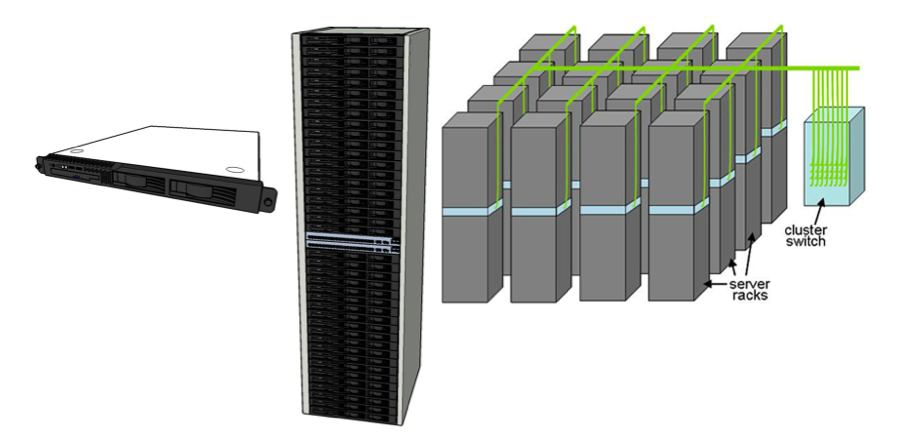
\includegraphics[width=0.7\textwidth]{images/racks} 
\caption{Organisation de racks. \cite{datacenterAsComputerIntro}}\label{racks}
\end{center}
\end{figure}

La figure \ref{racks} montre l'organisation des racks dans un data centre. Un serveur occupe 1 U du rack est montré à gauche. Au milieu on voit un rack et à droite un cluster de racks avec un swtich/routeur de niveau cluster. En général un ensemble de serveurs 1U sont montés dans un rack et inter-connectés avec commutateur Ethernet local. Ces switches au niveau des racks, qui peuvent utiliser des liens de 1 à 10 Gbps, ont un nombre de connexions montantes vers un ou plus switches de niveau cluster (data centre).

Le stockage dans les data centre peut être proposé de diverses manières. Souvent le stockage de haute performance est logé dans des \og  tours de stockage \fg{} qui permettent un accès distant transparent au stockage, indépendamment du nombre et des types des dispositifs de stockage physiques installés. Le stockage peut également être fourni dans une \og  brique de stockage \fg{} plus petite, localisée dans le rack ou slot de châssis ainsi que directement intégrée aux serveurs. Dans tous les cas, un accès réseau efficace au stockage est crucial.

Le problème le plus important dans cette structure est la potentielle insuffisance de bande passante. En général, les connexions montantes sont conçues pour supporter un certain taux de demandes excédentaires puisque la fourniture d'une bande passante entière n'est pas toujours possible. Par exemple, 20 serveurs à 1Gbps chacun doit partager un lien Ethernet montant unique de 10Gps à un taux de demande excédentaire de 2. Cette situation peut être problématique si la charge réseau non locale monte considérablement. Comme le stockage est traditionnellement fourni dans une tour séparée, tout le trafic de stockage traverse le lien montant dans le réseau stockage. Par exemple, l'archivage d'un gros volume peut consommer une importante bande passante. À mesure que les data centres augmentent en taille, une architecture réseau plus extensible devient essentielle.

La consommation d'énergie est également une des préoccupations de la conception des data centres, car les coûts liés sont devenus une part importante de la totalité des coûts pour cette classe de systèmes. Actuellement les CPUs ne sont plus le seul élément cible d'amélioration de l'efficacité énergétique, car ils ne dominent plus la majorité de la consommation. Des problématiques de ventilation et surconsommation d'énergie sont des facteurs de plus en plus critiques dans la conception de data centres.\cite{datacenterAsComputerIntro} \cite{dataCenterEvolution}

\section{Virtualisation et partage de ressources}

Le besoin d'augmenter l'efficacité dans l'utilisation des ressources a conduit à une conception d'infrastructures avec partage de ressources et virtualisation. La virtualisation fait référence à l'abstraction des ressources logiques de leurs couches physiques pour améliorer l'agilité, la flexibilité et la réduction des coûts et ainsi privilégier le business. La virtualisatoin permet de consolider un ensemble de composants d'infrastructures sous-utilisés en un nombre de dispositifs plus petits et mieux utilisés, contribuant à l'économie des coûts.

La virtualisation de serveurs est une méthode pour abstraire le système d'exploitation de la plateforme matérielle. Cela permet aux multiples systèmes d'exploitation ou multiples instances du même système d'exploitation de coexister dans un ou plusieurs processeurs. L'image \ref{virtinfra} illustre le partage de ressources par l'intermédiaire de la virtualisation.

\begin{figure}[h]
\begin{center}
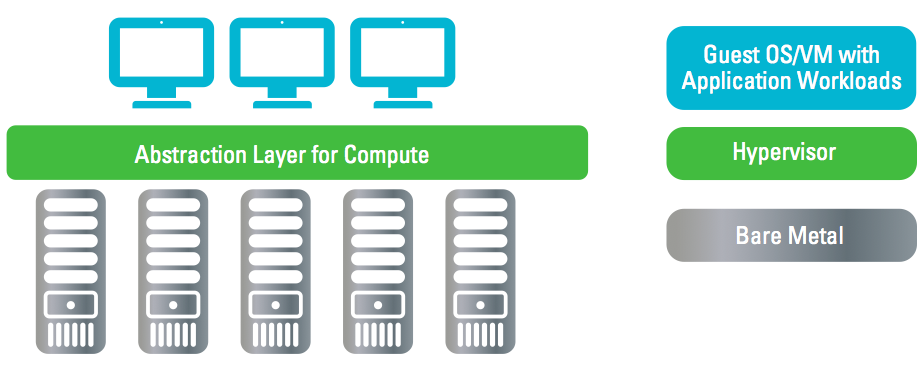
\includegraphics[width=0.98\textwidth]{images/shared_infa_virt} 
\caption{Modèle d'infrastructure à ressources partagées. \cite{journeySDDC}}\label{virtinfra}
\end{center}
\end{figure}

Un hyperviseur ou moniteur de machines virtuelles est inséré entre le système d'exploitation et le matériel pour réaliser la séparation entre le logique et le physique. Les instances de systèmes d'exploitation lancées sont appelées invités, ou systèmes d'exploitation invités. L'hyperviseur fournit l'émulation matérielle aux systèmes invités et gèrent l'allocation de ressources matérielles.  

%Ce modèle apporte des avantages en termes de comment les ressources sont efficacement utilisées avec des charges applicatives idéales.
Ce modèle apporte des avantages pour l'efficacité dans l'utilisation de ressources avec des charges applicatives idéales.
 Cependant, quand une application commence à consommer plus de ressources que l'estimé, il peut arriver des scénarios où les systèmes d'exploitation invités n'ont pas assez de ressources, impactant ainsi la qualité du service business offert. 

Cette approche a apporté une maitrise globale de management, monitoring et outillage. Elle a aussi mis en évidence que le composant \og compute \fg{} de l'infrastructure améliore clairement l'utilisation et automatisation des ressources serveurs. Cette amélioration a été possible grâce à la programmation du contrôle de ressources fournies aux instances invitées. Toutefois, le développement de nouvelles solutions pour gérer la charge dynamique de certaines application faisait toujours défaut. \cite{ibmPlanningVirtCCchap2}\cite{journeySDDC}

%This model has its advantages in terms of how resources are efficiently utilized in ideal applica- tion workloads. However, when one or more appli- cation workloads begin to consume more resourc- es than expected, scenarios could arise where several guest operating systems are short of compute resources, thereby impacting business application service level agreements.
%While this approach brought holistic capacity management, monitoring and tools capabilities, it also provided evidence that infrastructure compute and server resources were truly ben- efiting from improved resource utilization and automation. This was brought about, to a certain extent, by programmatically controlling the resources provided to guest instances. However, new thinking about solutions was still needed to meet the challenges of dynamic workloads of run- the-business applications and compute-intensive enterprise applications.



\section{Le besoin d'un modèle plus dynamique}


Traditionnellement, les data centres d'entreprises sont conçus pour durer pour toujours et atteindre les objectives visibles de l'économie. Cela veut dire que les éléments sous-jacents sont dimensionnés et construits pour supporter le pic de charge projeté en termes de performance, disponibilité et sécurité. Quand la croissance volumétrique projetée ne correspond pas à la réalité, cette méthode de dimensionnement peut conduire à une situation de sous-dimensionnement ou sur-dimensionnement. Ce qui apporte un effet négatif pour les investissements et les effort de réduction de coûts.

En général, pour atteindre une meilleure disponibilité, les infrastructures sont amenées à une sous-utilisation des ressources. Comme la charge des applications varient continuellement dans les applications sur internet, il reste deux choix : soit sous-dimensionner la provision et perdre des clients ou alors sur-dimensionner et gaspiller les ressources. 

Dans tous les cas, un plan détaillé de capacité est fait pour spécifier une série d'investissements importants en matériel et logiciel, dont la capacité est déterminée. L'image suivante illustre cette planification et les situations de problèmes de dimensionnement.


\begin{figure}[h]
\begin{center}
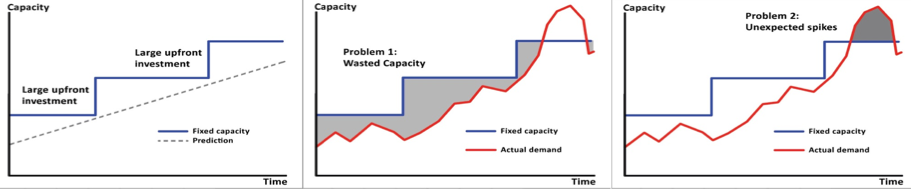
\includegraphics[width=0.98\textwidth]{images/fixed_capacity_load_prediction} 
\caption{Capacité fixe de ressources vs charge prévisionnelle. \cite{awsScaling}}
\end{center}
\end{figure}

Face à cette problématique, un nouveau mode de livraison a été proposé pour aborder les défis du traitement des demandes pour la variation dynamique des charges applicatives. Avec la nouvelle tendance du Cloud Computing et l'infrastructure en tant que service (IaaS), la conception de clusters hautement disponibles et des solutions extensibles peut être architecturée avec des requis non-fonctionnels comme base. 
%With the emergence of the cloud, the new age “mantra” and infrastructure as a service (IaaS) as a delivery model (as illustrated in Figure 3), the challenges of processing demands from dynamic workloads is being addressed. Designing high- availability clusters and scalable solutions can be architected based on nonfunctional requirements.

Avec sa nature extensible, le modèle de livraison cloud permet aux ressources d'être étendues et réduites  dynamiquement en fonction de la consommation. Une couche logicielle d'abstraction, implémentée par les hyperviseurs, virtualise le traitement des ressources physiques,  permettant ainsi au processeur, à la mémoire et aux disques durs de s'accommoder aux variations des demandes. \cite{awsScaling} \cite{journeySDDC}

%One of the biggest technical challenges of running an online business is how well they are able to handle the scalability requirements.  The Load traffic pattern keeps varying for online businesses and accordingly they will have to scale and maintain the acceptable performance levels.  Since the Traffic patterns are fluctuating in online business, they either tend to under provision and loose customers (or) over provision and waste hardware + costs. This problem is well illustrated in the below diagrams.
%Business usually makes detailed capacity planning and large upfront investment in their hardware and software. This HW/SW’s are usually provisioned with fixed capacity.

%Traditionally, enter-prise data centers are designed to last forever and meet visible business objectives, meaning that their underlying components are sized and built for a projected workload. They are also sized and built using application volumetric modeling and nonfunctional requirements such as perfor-mance, availability, scalability and security.

%The infrastructure is designed and provisioned considering the specific volumetric for support- ing the business applications and considering the peak load transaction in jobs per second, avail- ability and scalability requirements. When volu- metric and projected growth do not manifest as envisaged, this method of sizing infrastructure compute and storage could lead to either under- sizing or oversizing the footprint. Often, having such islands of infrastructure compute and storage leads to underutilization of resources. This has a cascading effect on investment and the effort expended toward energy consumption, management overheads, software licenses and data center costs.


%The shortcomings of this model led many enter- prises to the next wave of infrastructure design — utilizing shared infrastructure services and virtualized compute to increase efficiency in resource utilization and ensure that infrastruc- ture is designed and fit for the purpose, and not over-engineered.

%Virtualization refers to the abstraction of logical resources away from their underlying physical resources to improve agility and flexibility, reduce costs, and thus enhance business value. Virtualization allows a set of underutilized physical infrastructure components to be consolidated into a smaller number of better utilized devices, contributing to significant cost savings.

%Server virtualization is a method of abstracting the operating system from the hardware platform. This allows multiple operating systems or multiple instances of the same operating system to coexist on one or more processors. A hypervisor or virtual machine monitor (VMM) is inserted between the operating system and the hardware to achieve this separation. These operating systems are called “guests” or “guest OSs.” The hypervisor provides hardware emulation to the guest operating systems. It also manages allocation of hardware resources between operating systems.

%According to a recent Gartner study, the leading challenges facing today’s data centers are intrinsic to many of the aforementioned business drivers and their associated IT solutions. Top challenges cited include: 
%• Keeping up with data growth 
%• Maintaining system performance and scalability
%• Mitigating network congestion and connectivity issues
%• Minimizing power, cooling and space costs
%• Effectively managing the data center and its infrastructure
%Furthermore, according to a 2011 survey of the Data Center Users’ Group (DCUG), the leading infrastructure challenges included data center availability, high heat densities, energy efficiency and maintaining adequate power densities (see Figure 1). Each of these challenges resonates closely with the leading data center challenges faced by IT professionals.


%\section{Virtualisation}



%Integrated infrastructure solutions are specifically designed to provide advantages compared to a conventional physical infrastructure because they are: 
%•	 Efficient in power usage, space utilization and IT employee productivity
%•	 Economical in initial cost by making use of existing infrastructure and not requiring expensive room upgrades
%•	 Interoperable through simplified design and implementation of systems and components 
%•	 Controllable through planning, monitoring and management over the changing IT environment



%\section{Tendances des meilleures pratiques}


%Integrated infrastructure solutions are specifically designed to provide advantages compared to a conventional physical infrastructure because they are: 
%•	 Efficient in power usage, space utilization and IT employee productivity
%•	 Economical in initial cost by making use of existing infrastructure and not requiring expensive room upgrades
%•	 Interoperable through simplified design and implementation of systems and components 
%•	 Controllable through planning, monitoring and management over the changing IT environment
%\section{Architecture}

%\chapter{Cloud Computing}

% Un regard sur le nouveau \og business model \fg{} apporté par le Cloud Computing, les bénéfices de son adoption et les enjeux pour les infrastructures qui doivent répondre à ce nouveau paradigme, est l'objet de ce chapitre. Il sera démontré pour quelles raisons il nécessaires de faire évoluer les infrastructures actuelles vers le Cloud et pourquoi il n'est pas encore largement adopté.

\section{Cloud Computing}
En termes très simples, le Cloud Computing peut être défini comme un nouveau modèle de consommation et livraison de ressources de \gls{ti} et de services métiers, et est principalement caractérisé par :
\begin{itemize}
\item Libre service à la demande;
\item Service réseau très accessible;
\item Location indépendante de services en commun;
\item Extensibilité et approvisionnement rapides;
\item Paiement à la consommation.
\end{itemize}
%In very simple terms, cloud computing is a new consumption and delivery model for information technology (IT) and business services and is characterized by:
% • On-demand self-service
% • Ubiquitous network access
% • Location-independent resource pooling
% • Rapid elasticity and provisioning
% • Pay-per-use
Les avancements importants dans la virtualisation, réseau, approvisionnement et architectures multi-tenantes ont permis de faire évoluer radicalement les infrastructures de data centres. Le plus grand impact du Cloud Computing vient de l'instauration de nouveaux modèles de consommation et de livraison de services qui supportent l'innovation du business.

%Cloud has evolved from on demand and grid computing, while building on significant advances in virtualization, networking, provisioning, and multitenant architectures. As with any new technology, the exciting impact comes from enabling new service consumption and delivery models that support business model innovation.


L'évolution des data centres a permis de rendre service à une plus grande variété de besoins dans le monde du travail, ce qui implique la prise en compte de plusieurs facteurs lors de la conception face à différents objectifs. Le Cloud Computing est donc né en tant que nouveau paradigme pour les architectures data centre.

%As we have seen, data centers have grown to serve a wide range of business needs, and there are many factors to consider when designing a solution that meets different objectives. Within the past several years, a powerful new paradigm has emerged that has important implications for data center architectures and how they meet these varied objectives. This is the paradigm of cloud computing.

Le Cloud Computing livre dynamiquement des services sur des réseaux à partir d'un ensemble abstrait de ressources. Ces ressources se retrouvent quelque part dans le \og nuage \fg{} (symbole qui fait allusion à la représentation d'internet dans les topologies réseau) disponibles immédiatement à la demande. Les types de ressources ainsi que leur localisation sont transparents aux utilisateurs finaux. Ces utilisateurs se soucient principalement que leurs applications, données et contenus soient sécurisés et disponibles, avec un niveau de qualité spécifié.

%Cloud computing delivers services dynamically over networks from an abstracted set of resources. The resources are somewhere in the cloud and available on demand. The types of resources and their location are transparent to end users. End users primarily care that their applications, data and content are secure and available, with a desired level of quality.

Du point de vue de l'infrastructure, le Cloud Computing fait des fortes demandes aux ressources mutualisées dans une variété de technologies (de compute, de stockage, de réseau) pour leur allocation dynamique. Tout ceci dans un environnement automatisé, orchestré et logiquement diversifié, en conciliant une variété d'applications. L'orchestration permet de mutualiser les ressources à travers multiples data centres pour une réponse dynamique aux besoins clients. 


La virtualisation de serveurs a représentée un premier et important pas à la viabilisation de l'approche Cloud Computing. Toutefois, les autres deux éléments de base de l'infrastructure data centre doivent accompagner ces changements pour qu'on puisse avoir un accès complet aux services offerts par le Cloud. Plus spécifiquement la couche d'abstraction assurée par les hyperviseurs qui ont permis la séparation des systèmes logiques des serveurs physiques dans le cas de la virtualisation de serveurs doit être également appliquée aux matériels réseaux et de stockage. Cela permettra la définition d'un data centre entièrement piloté par du logiciel qui gère les ressources physiques les activant selon la charge applicative spécifiée à assurer.

L'abstraction de ces trois composants matériels est essentielle pour achever le mode de livraison cloud au sein des data centres. La virtualisation des serveurs a déjà atteint son adoption grand public, en 2009 un sondage avait trouvé que 77\% répondant déployait au moins un système virtualisé dans leur data centre \cite{x86ServersVirtualization}. Il se déroule actuellement beaucoup de travail en recherche et développement pour acquérir un niveau équivalent de maturité pour les dispositifs réseau et stockage. 

L'abstraction du stockage signifie la capacité à mutualiser les dispositifs physiques de stockage pour pouvoir les utiliser en tant que volumes de stockage logiques. Cela caractérise la virtulisation du stockage ou le \gls{sds}. Pour l'aspect stockage, il est connu que des solutions \gls{sds} se trouvent disponibles dans le marché, tels que EMC ViPR, HP StoreVirtual, IBM SmartCloud Virtual Storage Center entre autres.

De manière similaire, pour les réseaux il se développe une technologie fournissant une couche d'abstraction pour divers dispositifs réseau pour permettre l'isolation logique et indépendances du matériel. Il se trouve que \gls{sdn} est une des approches proposées pour traiter la problématique de l'abstraction réseau et fait donc l'objet de cette étude. Le chapitre suivant démontrera pour quoi les réseaux traditionnels ne sont pas adaptés aux exigences du Cloud Computing et analysera des exemples sur divers problèmes rencontrés. L'approche SDN et ses apports seront détaillés par la suite.
\cite{ibmPlanningVirtCCchap1}  \cite{cloudReadyJuniperReferenceDef} \cite{journeySDDC}

%From the infrastructure perspective, cloud computing heavily leverages resource pools in a variety of technologies— compute, storage and network—for dynamic allocation in an automated, orchestrated and logically diversified environment, accommodating a variety of applications. Using orchestration, resources can be pooled within and across multiple data centers to provide an environment that responds dynamically to user needs.

%\section{Besoins qui amènent au Cloud}

%Information technology (IT) is at a breaking point, and there is a critical need to improve IT's impact on the business.9
%Consider the following:
% -As much as 85\% of computing capacity sits idle in distributed computing environments.
% -Seventy percent of IT budgets is typically spent on maintaining current IT infrastructures, and only 30\% is typically spent on new capabilities.
% -Over 30\% of consumers notified of a security breach will terminate their relationship with the company that contributed to the breach.
%Clearly, infrastructures need to be more dynamic to free up budgets for new investments and accelerate deployment of superior capabilities being demanded by the business. Nearly all CEOs are adapting business models; cloud adoption can support these changing business dynamics.

%Functional Areas in the Cloud-Ready Data Center
%• Network Infrastructure—provides connectivity and transport for applications and services between users and the data center, within the data center and across multiple data centers. The Network infrastructure has three main sub components, namely the access network, the core network and the edge network.
%• Compute and Storage—represents the compute and storage infrastructure appropriate for applications (rack-mount and chassis-based, cost-effective and multi-core, with unstructured content and highly structured transaction databases). The compute and storage functional area hosts all business applications such as Enterprise Resource Planning (ERP), SaaS, SOA and Web 2.0 applications (among others).
%• Services—supports applications with security, user verification, and entitlement, and application support, including application acceleration, deep packet inspection (DPI), and load balancing
%• Management and Orchestration—ties together all of the elements of the cloud-computing infrastructure, enabling efficient and responsive monitoring, management, and planning

%\section{Nouveau business model}

%Even within the cloud computing space there is a spectrum of offering types. There are five commonly used categories:
%•  Storage as a Service - SaaS Provisioning of database-like services, billed on a utility computing basis, for example, per gigabyte per month.
%•  Infrastructure as a Service - IaaS Provisioning of hardware or virtual computers where the client has control over the OS, therefore allowing the execution of arbitrary software.
%•  Platform as a Service - PaaS Provisioning of hardware and OS, frameworks and databases, for which developers write custom applications. There will be restrictions on the type of software they can write, offset by built-in application scalability.
%•  Software as a Service - SaaS Provisioning of hardware, OS, and special-purpose software made available through the Internet.
%•  Desktop as a Service - DaaS Provisioning of the desktop environment, either within a browser or as a Terminal Server.

%\section{Principaux avantages du Cloud Computing}
%Key benefits of cloud computing:
%• Flexibility – There is the ability to update hardware and software quickly to adhere to customer demands and updates in technology.
%• Savings – There is a reduction of capital expenditures and IT personnel.
%• Location \& Hardware Independence – Users can access application from a web browser connected anywhere on the internet.
%• Multi-tenancy – Resources and cost are shared among many users, allowing overall cost reduction.
%• Reliability – Many cloud providers replicate their server environments in multiply data centers around the globe, which accounts for business continuity and disaster recovery.
%• Scalability – Multiply resources load balance peak load capacity and utilization across multiply hard- ware platforms in different locations
%• Security – Centralization of sensitive data improves security by removing data from the users’ com- puters. Cloud providers also have the staff resources to maintain all the latest security features to help protect data.
%• Maintenance – Centralized applications are much easier to maintain than their distributed counter parts. All updates and changes are made in one centralized server instead of on each user’s computer.


%\section{Barrières au Cloud Computing}

%IT organizations have identified four major barriers to large-scale adoption of cloud services:
%•  Security, particularly data security
%Interestingly, the security concerns in a cloud environment are no different from those in a traditional data center and network. However, since %most of the information exchange between the organization and the cloud service provider is done over the web or a shared network, and %because IT security is handled entirely by an external entity, the overall security risks are perceived as higher for cloud services.
%Some additional factors cited as contributing to this perception:
%– Limited knowledge of the physical location of stored data
%– A belief that multitenant platforms are inherently less secure than single-tenant platforms
%– Use of virtualization as the underlying technology, where virtualization is seen as a relatively new technology
%– Limited capabilities for monitoring access to applications hosted in the cloud
%•  Governance and regulatory compliance
%Large enterprises are still trying to sort out the appropriate data governance model for cloud services, and ensuring data privacy. This is particularly significant when there is a regulatory compliance requirement such as SOX or the European Data Protection Laws.
%•  Service level agreements and quality of service
%Quality of service (availability, reliability, and performance) is still cited as amajor concern for large organizations:
%– Not all cloud service providers have well-defined SLAs, or SLAs that meet stricter corporate standards. Recovery times may be stated as “as soon as possible” rather than a guaranteed number of hours. Corrective measures specified in the cloud provider's SLAs are often fairly minimal and do not cover the potential consequent losses to the client's business in the event of an outage.
%– Inability to influence the SLA contracts. From the cloud service provider's point of view it is impractical to tailor individual SLAs for every client they support.
%– The risk of poor performance is perceived higher for a complex cloud-delivered application than for a relatively simpler on-site service delivery model. Overall performance of a cloud service is dependent on the performance of components outside the direct control of both the client and the cloud service provider, such as the network connection.1. Integrationandinteroperability
I%dentifying and migrating appropriate applications to the cloud is made complicated by the interdependencies typically associated with business applications. Integration and interoperability issues include:
%– A lack of standard interfaces or APIs for integrating legacy applications with cloud services. This is worse if services from multiple vendors are involved.
%– Software dependencies that must also reside in the cloud for performance reasons, but which may not be ready for licensing on the cloud.
%– Interoperability issues between cloud providers. There are worries about how disparate applications on multiple platforms, deployed in geographically dispersed locations, can interact flawlessly and can provide the expected levels of service.



\chapter{L'aspect réseau}
Dans ce chapitre, les principales problématiques data centre dans un aspect réseau seront présentées et analysées.  Comment on fait aujourd'hui ? Quels sont les limites ? 


\section{Le réseau dans un data centre}

Avec la prise des projets d’optimisation de \gls{ti} tels que la consolidation de data centre et la virtualisation de serveur, une attention spéciale doit être prise au rôle critique des réseaux dans la planification, exécution et succès en général du projet. Il souvent admet que des planifications supplémentaire par rapport aux réseaux auraient pu contribuer pour le succès de plusieurs projets.

%As organizations undertake information technology (IT) optimization projects, such as data center consolidation and server virtualization, they need to ensure that the proper level of focus is given to the critical role of the network in terms of planning, execution, and overall project success. While many consider the network early in the planning stages of these projects and spend time considering this aspect of these initiatives, many more feel that additional network planning could have helped their projects be more successful.


Les principaux types de changements réseau dans les projets d'optimisation TI incluent l'implémentation d'équipement réseau supplémentaire pour augmenter la redondance, l'augmentation de la capacité du réseau avec la modernisation de switchs, l'amélioration de la sécurité réseau et l'augmentation de la bande passante. Cependant, plusieurs requis associés à ces changement l'initiative en général sont pas identifiés tout de suite au début du projet. Très souvent ils ne sont pas détectés qu'après les étapes initales du projet, imposant un supplément de travail et l'ajout des coûts non anticipés.

%The most common types of network changes in IT optimization projects include implementing new network equipment, adding greater redundancy, increasing capacity by upgrading switches, improving network security, and adding network bandwidth. However, many network requirements associated with these changes and the overall initiative are typically not identified until after the initial stages of the project and often require rework and add unanticipated costs. Regardless of project type, network challenges run the risk of contributing to increased project time lines and/or costs.


The networking aspects of projects can be challenging and user complaints about the network are frequently heard. Important challenges include the inability to perform accurate and timely root-cause analysis, understand application level responsiveness, and address network performance issues. Simply buying more network equipment does not necessarily or appropriately address the real requirements.


Looking ahead, many expect that the network will become more important to their companies' overall success. To address this, networking investments related to support of server and storage virtualization are currently at the top of the list for consideration, followed by overall enhancement and optimization of the networking environment.
To support virtualization of the entire IT infrastructure and to continue to optimize the network, IT organizations need to make architectural decisions in the context of the existing infrastructure, IT strategy, and overall business goals.


Developing a plan for the network and associated functional design is critical. Without a strong plan and a solid functional design, networking transitions can be risky, leading to reduced control of IT services delivered over the network, the potential for high costs with insufficient results, and unexpected performance or availability issues for critical business processes.


With a plan and a solid functional design, the probability of success is raised: a more responsive network with optimized delivery, lower costs, increased ability to meet application service level commitments, and a network that supports and fully contributes to a responsive IT environment.

\section{Challenges réseau}

Unified Fabric

If one studies a typical data center server infrastructure, it is easy to notice that servers have a series of network interfaces connected to multiple types of networks (LAN, SAN, IPC). This arrangement adds complexity in the form of cost, cabling, port count, scalability, power, and cooling. If we follow the same tradition in a cloud data center, this architecture will not scale to the density that is typically expected. Hence, to continue to reduce the total cost of ownership (TCO) and to deploy virtual machines, all servers must have a consistent and ubiquitous set of network and storage capabilities. One of the simplest and most efficient ways to deliver these capabilities is to deploy a unified fabric. The shift to a unified fabric gives all servers (physical and virtual) access to the LAN, SAN, and IPC networks, allowing more to be consolidated in the customer’s network for greater efficiency and costs savings.

Cisco is offering not only 10 Gigabit Ethernet, but also lossless 10 Gigabit Ethernet, currently called Data Center Ethernet or Enhanced Ethernet. This becomes the foundation to consolidate fabrics like Fiber Channel (for SAN), which require the stringent lossless nature of a network. Fibre Channel over Ethernet (FCoE), which is a standard accepted by standard bodies and industry, is leading the way to unify fabric on a cloud data center. Hence, to consolidate server I/O, the server access layer must be adapted to support a unified fabric. Additionally, a new breed of adapters, called converged network adapters (CNAs), would be implemented in the server platform, which will act at the consolidation and virtualization point in the compute layer.


Cisco believes that the network platform is a foundational component of a utility service platform as it is critical to providing intelligent connectivity within and beyond the data center. With the right built-in and external tools, the network is ideally placed to provide a secure, trusted, and robust services platform.

The network is the natural home for management and enforcement of policies relating to risk, performance, and cost. Only the network sees all data, connected resources, and user interactions within and between clouds. The network is thus uniquely positioned to monitor and meter usage and performance of distributed services and infrastructure. An analogy for the network in this context would be the human body’s autonomic nervous system (ANS) that acts as a system (functioning largely below the level of consciousness) that controls visceral (inner organ) functions. ANS is usually divided into sensory (affer- ent) and motor (efferent) subsystems that is analogous to visibility and control capabili- ties we need from a services platform to derive a desired outcome. Indeed, at the time of this writing, there is a lot of academic research into managing complex network systems, might they be biological, social, or traditional IT networking. Management tools for the data center and wider networks have moved from a user-centric focus (for example, GUI design) to today’s process-centric programmatic capabilities. In the future, the focus will most likely shift toward behavioral- and then cognitive-based capabilities.

The network also has a pivotal role to play in promoting resilience and reliability. For example, the network, with its unique end-to-end visibility, helps support dynamic orchestration and redirection of workloads through embedded policy-based control capabilities. The network is inherently aware of the physical location of resources and users. Context-aware services can anticipate the needs of users and deploy resources appropriately, balancing end-user experience, risk management, and the cost of service.


\section{Différents usages}

\section{Agilité}

\section{Sécurité}

introduction
Some security risks unique to a virtualization infrastructure include communication blind spots, inter-VM attacks, and mixed trust level VMs. Instant-on gaps and resource contention are also important considerations. This section addresses each of these threats and issues.

communication Blind Spots

In virtualized environments, traditional network security appliances are blind to the communication between VMs on the same host unless all communications are routed outside the host machine to this separate appliance. But this security configuration introduces significant time lags. One way to eliminate blind spots while reducing time lags is to place a dedicated scanning security VM on the host that coordinates communication between VMs. This solution works well in a virtualized environment. However, a dedicated security VM is not ideal for a cloud environment. The dedicated security VM integrates with the hypervisor to communicate with other guest VMs. In some cloud environments, such as in a multi-tenant public cloud, users do not have access to the hypervisor. In the cloud, protection is best provided as self-defending VMs. Protection is self contained on each VM and does not require communication outside of the VM to remain secure.

inter-Vm attacks and hypervisor compromises

Virtualized servers use the same operating systems, enterprise applications, and web applications as physical servers. Hence, the ability of an attacker to remotely exploit vulnerabilities in these systems and applications is a significant threat to virtualized environments as well. And once an attacker compromises one element of a virtual environment, oather elements may also be compromised if virtualization-aware security is not implemented.
In one scenario, an attacker can compromise one guest VM, which can then pass
the infection to other guest VMs on the same host. Co-location of multiple VMs
increases the attack surface and risk of VM-to-VM compromise. A firewall and an intrusion detection and prevention system need to be able to detect malicious activity at the VM level, regardless of the location of the VM within the virtualized environment.

Another attack mode involves the hypervisor, which is the software that enables multiple VMs to run within a single computer. While central to all virtualization methods, hypervisors bring both new capabilities and computing risks. A hypervisor can control all aspects of all VMs that run on the hardware, so it is a natural security target. Therefore, securing a hypervisor is vital, yet more complex than it seems.

In an attack known as “hyperjacking,” malware that has penetrated one VM may attack the hypervisor. When a guest VM attempts this attack, it is often called a “guest VM escape” because the guest VM breaks out of, or escapes, its isolated environment and attacks the host hypervisor. Once compromised, a hypervisor can then attack other guest VMs on that host.

VMs make requests to the hypervisor through several different methods, usually involving a specific application programming interface (API) call. An API is the interface created to manage VMs from the host machine. These APIs are prime targets for malicious code, so virtualization vendors attempt to ensure that APIs are secure and that VMs make only authentic (i.e. authenticated and authorized) requests. Because this is a critical path function, speed is a significant requirement in all hypervisors to ensure that overall performance is not impeded.
When attackers targeted a zero-day vulnerability in a virtualization application called HyperVM made by LXLabs, as many as 100,000 web sites were destroyed [1]. In addition, certain virtualization vendors like Amazon Web Services have made their APIs public. These will undoubtedly become interesting targets for cybercriminals. Vendors that have not made their APIs public like vSphere, while not usually externally exposed, can also become potential targets for attacks within their perimeters. There is a risk that, owing to the rapid change in the API space and the current race to market, virtualization management systems will not be secure in the future.

mixed trust level Vms

VMs with mission-critical data may reside on the same host as VMs with less critical data – resulting in mixed trust level VMs. Enterprises can attempt to segregate these different levels of secure information on separate host machines, but in some cases, this can defeat the purpose of a virtualized environment – to make the most efficient use of resources. Enterprises need to ensure that mission-critical information is protected while still realizing the benefits of virtualization. With self-defending VM security, VMs can remain safe even in mixed trust level environments, with protection such as intrusion detection and prevention, a firewall, integrity monitoring, log inspection, and antivirus capabilities.

instant-on gaps

Virtualized environments are not necessarily inherently less secure than their physical counterparts. However, in some cases, the practical uses of virtualization can introduce vulnerabilities, unless administrators are aware of these vulnerabilities and take steps to eliminate them. Instant-on gaps are an example of such a vulnerability.
Beyond server consolidation, enterprises take advantage of the dynamic nature of VMs by quickly provisioning, cloning, migrating, and decommissioning VMs as needed, for test environments, scheduled maintenance, and disaster recovery, and to support task workers who need computational resources on-demand. As a result, when VMs are activated and inactivated in rapid cycles, rapidly and consistently provisioning security to those VMs and keeping them up-to-date can be challenging.

After a period of time, dormant VMs can eventually deviate so far from the baseline security state that simply powering them on introduces significant security vulnerabilities. And even if VMs are dormant, attackers may still be able to access them. Also, new VMs may be cloned from VM templates with out-of-date security. Even when VMs are built from a template with virus protection and other security applications, the VMs need the security agent to have the latest security configurations and pattern file updates.

When dormant, reactivated, or cloned VMs have out-of-date security, attackers may be able to leverage an exploit for a longer period of time – the attack may have more longevity. Generally, if a guest VM is not online during the deployment or updating of antivirus software, it will lie dormant in an unprotected state and be instantly vulnerable when it does come online. One solution is a dedicated security VM on each host that automatically updates VMs with the latest security when activated or cloned, and safely allows enterprises to realize the benefits of virtualization.

resource contention 

%When resource intensive operations such as regular antivirus scans and pattern file updates designed for physical environments are applied to VMs, these operations can quickly result in an extreme load on the system. When antivirus scans or scheduled updates simultaneously kick into action on all VMs on a single physical system, the result is an antivirus storm. This storm is like a run on the bank, where the bank is the underlying virtualized resource pool of memory, storage, and CPU. This performance impact hampers server applications and VDI environments.

The legacy security architecture also results in linear growth of memory allocation as the number of VMs on a single host grows. In physical environments, antivirus software must be installed on each operating system. Applying this architecture to virtual systems means that each VM requires additional significant memory footprint  an unwanted drain on server consolidation efforts.
Products that are not virtualization-aware suggest the use of randomization or grouping to avoid resource contention.

However, randomization does not help to avoid times of high system usage and requires that a long period of time be reserved for the full scan cycle. Grouping does not allow for the mobile nature of virtualization, requiring reconfiguration when VMs are migrated or cloned.




%\chapter{Enjeux de SDN}

Ce chapitre présente quels sont les enjeux pour déployer SDN. Il a pour but d'identifier les challenges lors de la mise en place de cette architecture ainsi que les problèmes susceptibles d'être rencontrés. Pour chaque enjeux, les idées pour les surmonter sont montrées tout en proposant les compromis de ces solutions.

\section{Contrôle : centralisé ou distribué}
Contrôle centralisé = un seul point de faille pour le réseau complet.

Architecture physiquement distribuée mais centralisé au niveau logique.

Consistence et stateliness quand on distribue des états sur le réseau peut causer un mal comportement des applications qui pensent qu'elles une vision précise du réseau.

\section{Niveau de granularité}

\section{Politiques : réactives ou pro-actives}

\section{Fonctions de Virtualisation du Réseau}
%\gls{nfv}

\chapter{Applications SDN et leurs apports aux data centres}

Ce chapitre définira SDN et présentera les réponses aux problématiques réseau rencontrées en général dans les data centres et qui ont été débattues dans le chapitre précédent. %Comment SDN approche la problématique ? Qu'est-ce que SDN ?
%Le chapitre démontrera également les apports de SDN au sein des data centres par rapport à ces problématiques présentées précédemment.

\section{Définition de SDN}

Les pré-requis réseaux des applications devraient être articulés dans un langage simple, utilisé pour demander les comportements réseau souhaités. La  programmation des réseaux est aujourd'hui très limitée, introduisant un malheureux compromis : obligation de développer les applications par un paramétrage réseau excessivement détaillé, ou ignorer de ces détails par le traitement du réseau comme une boîte noire.
%le développement d'applications contraint par un paramétrage réseau excessivement détaillé, ou l'ignorance de ces détails par le traitement du réseau comme une boîte noire. 
Aucune de ces solutions n'est convenable ; la première implique des applications spécifiques à chaque type de réseau alors que dans la deuxième, le contrôle nécessaire %à l'extraction de fonctionnalités réseau 
n'est pas présent. 
%The definition of network services must be application-centric and simple. The networking requirements of applications should be articulated in an IT-friendly language and used to request desired network behaviors. Today there is limited programmability, resulting in an unfortunate tradeoff. Engineering of cloud applications is either encumbered by detailed network-specific parameters and information, or ignores them and treats the network as a “black box”. Neither is optimal. The first option leads to custom applications for each network type while with the second, applications lack the visibility and control needed to leverage the true capabilities of the network.

Un niveau approprié  d'abstraction\index{Abstraction} des réseaux est nécessaire pour les rendre programmables et améliorer l'utilisation des ressources. L’instanciation de services réseau doit pouvoir se faire instantanément, de manière alignée aux besoins des applications. Le réseau doit permettre l'établissement de connectivité interne et entre data centres, tout en gardant la cohérence avec les politiques (de sécurité, de disponibilité et de réglementation) définies par le prestataire cloud et ses tenants. Aujourd'hui, tout cela se fait lentement, manuellement avec un risque élevé d'erreurs, comptant sur les ordres de travail pour établir une  multitude  de configurations selon le fournisseur de chaque équipement.
%The proper abstraction of network capabilities, consistent with Software Defined Networking (SDN) principles, drives programmability of network services and increases the consumability of network resources. The instantiation of network services must be instantaneous, aligned with the needs of applications. The network should act reflexively to establish the required connectivity within and across datacenters, and do so in a manner that is consistent with the defined policies of CSPs and their tenants. Today that process is slow, manual and error-prone, relying on work orders to establish a multitude of vendor- dependent configurations.

Les principes \gls{sdn} %sont plus adaptés à ce scénario, l'approche propose 
proposent une couche d'abstraction\index{Abstraction} pour permettre la programmation du réseau et autoriser le contrôle dynamique de services. SDN est un nouveau \gls{paradigme} réseau défini comme une architecture qui a pour but de centraliser  sur un contrôleur l'intelligence du réseau. Cette intelligence étant traditionnellement distribuée parmi plusieurs équipements réseaux réalisant une fonction spécifique dans l'infrastructure.

Ces dispositifs ont en général une fonctionnalité de commutation de paquets (\gls{dataplane}) et une partie de traitement des données en appliquant une logique spécifique selon les états et la configuration enregistrés (\gls{controlplane}). SDN propose de dissocier ces deux fonctions dans les dispositifs et d'agréger dans un contrôleur commun l'activité de traitement. L'image ci-dessous permet de visualiser les différences entre les architectures traditionnelle et SDN. \\


\begin{figure}[h]
\begin{center}
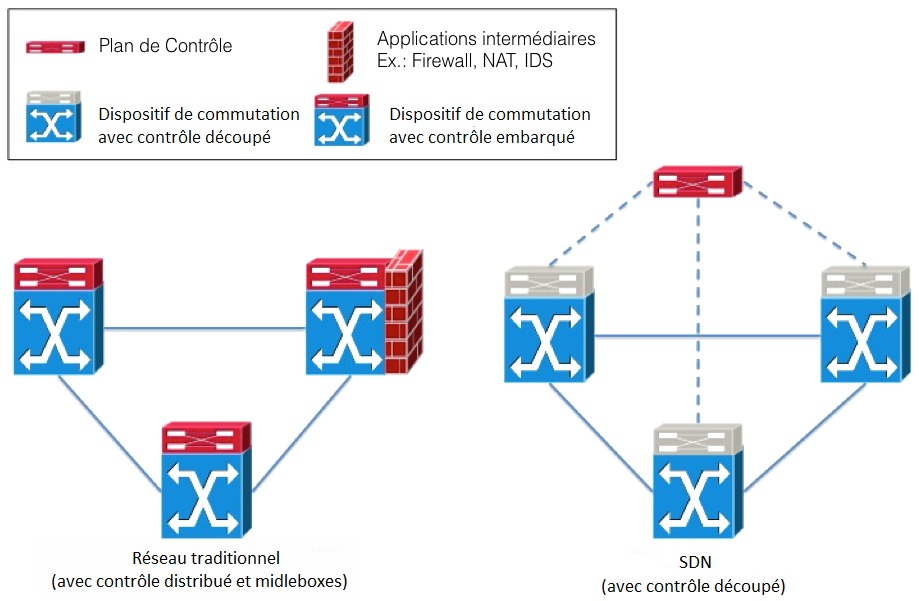
\includegraphics[width=0.7\textwidth]{images/TraditionalVsSDN} 
\caption{Architectures : réseau traditionnel et SDN. \cite{SurveySDNArchi}} \label{TraditionalVsSDN}
\end{center}
\end{figure}


L'expérience, lors de la construction des grands réseaux IP/MPLS, a montré que l'intelligence doit être poussée vers la périphérie pour autoriser la \gls{scalability}\index{Scalabilité} des réseaux. Le principe doit être appliqué afin de promouvoir un cœur du réseau data centre simplifié et efficace. L'approche sépare les services réseaux de l'infrastructure physique permettant l'innovation\index{Innovation} parallèle dans les deux domaines.

%Application of lessons learned from building very large IP/MPLS networks. In the “thin waist” model for scaling IP networks, intelligence is pushed to the edges. The same is in order for promoting a simple and cost-effective core datacenter network, consistent with the manner in which IP technologies have successfully scaled to date. The approach decouples network services from the infrastructure and enables parallel innovation in each domain.

Les leçons acquises lors de la conception des réseaux mobiles ont apporté la technique d'optimisation pour la mobilité et d'automatisation opérationnelle à large échelle. Cela permet la création d'un modèle auto-instancié et dirigé selon les règles établies qui minimise les coûts d'implémentation et délais de livraison de service\index{Mode de livraison}.
%Application of lessons learned from design of mobile networks that have been optimized to provide mobility and operational automation at massive subscriber scale. This yields a policy-driven auto-instantiation model for the datacenter network that minimizes costs and delays. The new model significantly changes the game, greatly increasing the efficiency with which cloud services canbe delivered.

%En complément de ces principes, SDN propose également une interface commune de programmation du réseau sous-jacent, grâce à l'abstraction de ses capacités.
%Bringing common IT language to programming the underlying network by abstracting the network capabilities into IT and business logic terminology.

Cette solution apporte comme bénéfice l'introduction d'une interface commune et programmable de management, permettant la mise en place dynamique de services, indépendamment de la marque/modèle des dispositifs réseau. Avec SDN, l'administration réseau devient plus agile\index{Agilité} car un seul élément (le contrôleur) est à maîtriser au lieu d'avoir à configurer l'ensemble des équipements du système, ce qui accélère considérablement le temps de convergence du réseau pour l'accommodation de nouvelles applications déployées. \cite{SDNNewNormONFExecutiveSummary} \cite{ImplementationChallengesForSDNBackground}





\section{Virtualisation des fonctions réseau, NFV}


Un concept qui est très souvent discuté en parallèle à \gls{sdn} est \gls{nfv}. \gls{nfv} pousse les technologies de virtualisation à consolider les applications réseau sur des serveurs, switches et baies de stockage\index{Stockage} standard de l'industrie. La virtualisation des fonctions réseau non seulement réduit les dépenses en équipements, mais aussi apporte d'autres bénéfices tels que l'extension\index{Scalabilité} agile\index{Agilité} d'applications, à une vitesse plus rapide, une plus haute disponibilité et une meilleure utilisation de ressources.
%A concept that often gets discussed in conjunction with SDN is Network Function Virtualization (NFV).
%NFV leverages standard virtualization technologies to consolidate network applications – which have traditionally been hosted on proprietary hardware appliances – onto industry standard servers, switches and storage. In addition to reducing expenditure on equipment costs, virtualizing network functions also brings benefits such as rapid scaling of applications, faster speed of innovation, increased high availability and improved resource utilization. 

Toutefois, pour bénéficier de ces apports, il est nécessaire que l'infrastructure réseau sous-jacente s'adapte rapidement et automatiquement. Par exemple, pour migrer une fonction réseau  dans un nouveau matériel, les politiques et les configurations associées à ce service doivent être provisionnées dans beaucoup d'autres équipements et fonctions. La complexité à configurer les réseaux dans un environnement si dynamique augmente énormément avec l'introduction de nouveaux éléments réseaux.
%However, realizing these benefits requires that the underlying network infrastructure is adapted quickly and automatically. For example, for a network function to either scale up or migrate onto a new piece of hardware, the security and policy configuration associated with that network function may have to be provisioned on a large number of switches and other network functions. The complexity of configuring networks in such a dynamic environment increases greatly as the number of network elements increase.


Bien que les développements de SDN et NFV puissent progresser indépendamment, l'association des deux principes est d'un fort intérêt pour le progrès des solutions cloud. SDN peut être employé en tant que technologie facilitatrice de la virtualisation des fonctions réseau, favorisant la consolidation des applications réseau dans des dispositifs industriels standard. \cite{OFSDNNFVintro} \cite{realTimeCloudNFV} \cite{IntelCloudEPC}

%Mainstream industry adoption and deployment of Cloud Telecoms will be hindered, or even blocked, until carrier grade telecom requirements have been fully proven on the key technologies underpinning the Cloud Telecoms concept, namely Network Functions Virtualisation (NFV), Software Defined Networking (SDN) and deployment on industry-standard, high- volume servers.
%While the development of SDN and the development of NFV can proceed independently, there are some areas of possible overlap and cooperation.

%When services are needed, these components are assembled (or orchestrated) and deployed on servers. The NFV plan is to support everything from bare metal to an architected cloud as a hosting platform. Once deployed, they are managed so as to create as good of a service experience as the original devices would have created.



\section{SDN, NFV et le Cloud Computing}

Les approches Cloud permettent aux opérateurs réseau d'assurer une création et un déploiement de services plus rapides. Elles répondent également aux attentes croissantes sur la qualité et la performance des solutions, tout en traitant les charges\index{Charge} trafics de plus en plus importantes.


%Cloud-based approaches enable network operators to ensure rapid service creation and rollout by delivering new levels of flexibility, scalability and responsiveness. They also satisfy the growing expectations for service performance and QoE, while handling ever-increasing traffic loads.Operators are making use of NFV, SDN and cloud technology in three ways:
%> Telecom cloud – operators are gradually turning their networks into layered and distributed clouds, in which workloads can be located to optimize QoE or data transport, and to offer the best possible elasticity.
%> IT cloud – operators are optimizing the use of internal IT resources to deliver an improved customer experience, to accelerate time to market for innovative and compelling services, and to improve their efficiency for cost reduction.
%> Customer cloud – operators leverage a platform, or their own cloud, to resell or broker value-added cloud services.
%Although these scenarios are all quite different, they share some common requirements, and operators can benefit from the implementation of a common platform across all three scenarios.

Afin de supprimer les contraintes des réseaux dans les data centres, une plateforme innovante\index{Innovation} pour l'abstraction\index{Abstraction} des fonctionnalités réseau et pour l'instanciation automatisée de services est proposée. Avec SDN, les fournisseurs de services cloud, opérateurs à l'échelle web et grandes entreprises technologiques peuvent construire une infrastructure réseau multi-tenante, robuste et extensible\index{Scalabilité} pour délivrer des espaces virtuels de compute\index{Virtualisation}, stockage\index{Virtualisation du Stockage} et réseau\index{Virtualisation du Réseau} prêts à l'usage pour des milliers de tenants et groupes d'utilisateurs.

%Nuage NetworksTM removes the constraints of the datacenter network through an innovative Virtualized Services Platform (VSP) that abstracts network capabilities and automates service instantiation. With the Nuage Networks Software Defined Networking solution, cloud service providers, web-scale operators and large tech enterprises can b uild a robust and scalable multi-tenant networking infrastructure that delivers secure virtual slices of readily consumable compute, storage and networking instantaneously across thousands of tenants and user groups.


%Combining a Network-enabled Cloud approach (which offers flexible management of cloud applications) with NFV (several virtualized applications on a common hardware platform, which reduces opex and capex) and the real-time control capabilities of Service Provider SDN (as shown in Figure 3) yields significant advantages. 
%First, it enables operators to more easily (and usually automatically) adapt network characteristics and resources to serve the more dynamic and real-time nature of new services. 
%Second, it extends the virtual infrastructure beyond the traditional computing and storage resources to enable applications to encompass WAN resources – making it easier to engage one or more data centers, as well as any other intelligent nodes in the network.
%Network-enabled Cloud delivers the flexibility and elasticity to deploy software applications and virtualized network functions wherever they are needed in the network. This improves time to market and enhances innovation, QoE and network efficiency.

Le \gls{controlplane} dans SDN fonctionne en lien avec le système de management cloud afin de configurer dynamiquement des éléments réseaux pour s'adapter aux décisions des systèmes d'orchestration pour le changement d'utilisations des ressources. SDN fournit l'infrastructure nécessaire pour réaliser cette capacité de NFV étendue.
%The control plane in software-defined networks works in conjunction with cloud management systems in order to dynamically configure network elements to adapt to changing resource usage decisions made by cloud orchestration systems. SDN provides the infrastructure required to truly realize the potential of NFV.

La figure \ref{cloud-sdn-nfv} affiche comment SDN et NFV s'intègrent dans une infrastructure Cloud pour atteindre les objectifs de virtualisation du réseau. \\

\begin{figure}[h]
\begin{center}
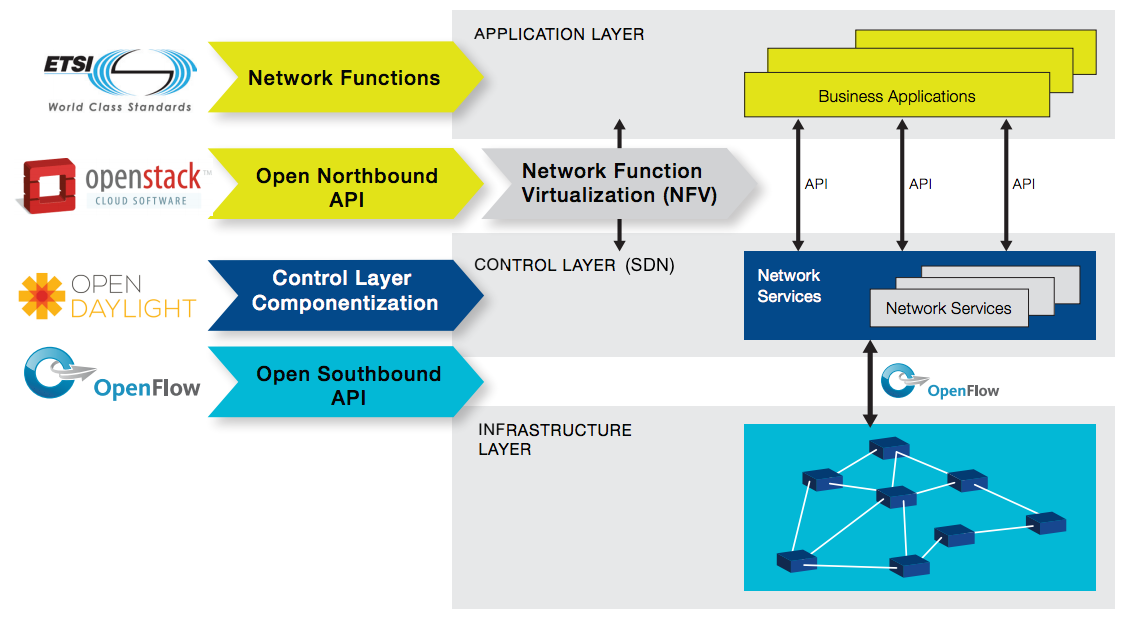
\includegraphics[width=0.8\textwidth]{images/cloud-sdn-nfv} 
\caption{SDN, NFV et Cloud Computing. \cite{OFSDNNFVand}} \label{cloud-sdn-nfv}
\end{center}
\end{figure} 

L'image montre également les protocoles et standards ouverts qui émergent pour chaque technologie comme \gls{openflow} pour la communication entre les dispositifs réseau et le contrôleur SDN (\gls{opendaylight}), OpenStack pour la gestion Cloud et ETSI pour le NFV. Il est important de noter que de grands noms de l’industrie (comme Cisco, Microsoft, Google etc.) se sont engagés dans ces projets pour accélérer le développement de ces technologies.

Dans le cloud, avec SDN et NFV travaillant ensemble, on peut dynamiquement étendre les fonctions réseau au sein des data centres. Par exemple, lorsque la charge\index{Charge} réseau augmente, le contrôleur SDN peut demander au gestionnaire cloud d'instancier une nouvelle fonction réseau dans le cloud pour redistribuer et répartir le trafic. 
%(pas claire) Another case that brings out the value of a combined real-time programmable network and cloud solution is the ability to dynamically extend network functions into the cloud – with SDN, NFV and the cloud all working together. As the load on a network appliance increases, the SDN controller can request a peer cloud manager to instantiate a virtual network function in the cloud and to start load balancing between the physical appliance and the virtual appliance, treating it as a common entity.

%However, fully realizing the potential of this technology in today’s service provider networks means doing more than just separating the forwarding and control planes. This expanded definition of Service Provider SDN includes:

%> Integrated network control – this unified control layer controls the data center and network as an integrated entity, in order to deliver the best user experience.
%> Orchestrated network and cloud management – a unified approach that includes legacy network management and new cloud management systems. It is this end-to-end orchestration that enables flexible service creation, which in turn makes the network dynamic, adaptive and agile. This cuts introduction and modification cycles for services and removes barriers to innovation.
%> Service exposure – the SDN architecture provides network awareness to the application layer through service exposure application programming interfaces (APIs). These APIs not only provide raw network data, but are instead composed APIs that deliver actionable information at the application level.

La couche de contrôle SDN apporte l'allocation de ressources extensible et en temps-réel pour les besoins des services réseaux. Cela permet que les services soient définis et provisionnés très rapidement via de portails libre services. Le service est mis à disposition dans un délai de minutes, au lieu de jours ou même semaines comme il est traditionnellement nécessaire.
%The service control layer of the Service Provider SDN architecture brings elastic, real-time allocation of resources for networking services. It enables these services to be defined and provisioned through self-service portals in a matter of minutes, rather than the days, weeks or even months that are traditionally required.

Cette plateforme, avec un contrôle intégré à travers des domaines réseaux, expose des \glspl{api} qui permettent aux applications d'instancier dynamiquement des ressources pour accomplir ces objectifs métiers. Un  système de management de l'infrastructure fournit des capacités supplémentaires, comme une planification plus fiable, approvisionnement, activation, adaptation et le contrôle de nouvelles connexions de services.
%This demands a platform with integrated control across networking domains that exposes “composed APIs” for new revenue generation. An end-to-end network management system across IP and transport infrastructure provides further efficiencies, develops greater responsiveness, and enables more reliable planning, provisioning, activation, adaptation and control of new service connections.

SDN permet de coupler la gestion du cloud au réseau programmable, achevant une intégration complète du réseau. Avec une orchestration commune des services, on obtient une réduction des coûts opérationnels pour l'approvisionnement et la supervision ainsi qu'une création flexible de services. Cela rend le réseau dynamique, adaptatif et agile\index{Agilité}, donc prêt pour le Cloud. \cite{OFSDNNFVand} \cite{realTimeCloudNetworkEnabled} 
%The goal is to couple cloud management to a programmable network, via SDN controllers, to achieve full integration of the cloud and network, where cloud resources are no longer confined to a single data center, but are spread throughout the network.

%Using common orchestration for end-to-end service management as well as for operations, administration and maintenance reduces operating costs in areas such as provisioning, monitoring and faultfinding. More importantly, end-to-end orchestration enables flexible service creation, which makes the network dynamic, adaptive and agile.

\chapter{Apports de SDN aux data centres}
Ce chapitre démontre les apports de SDN au sein des data centre par rapports aux problématiques présentées précédemment.

\section{Différents usages}

\section{Agilité}

\section{Sécurité}


\addchap{Conclusion}

%Même avec le succès incontestable de l'architecture d'internet, l'état de l'industrie réseau et l'essence de son infrastructure se trouvent en phase critique. Il est généralement admis que les réseaux courants sont excessivement chers, compliqués à gérer, sujets aux blocages des fournisseurs et difficiles à faire évoluer. 

Au sein des data centres, les technologies de virtualisation des serveurs ont évolué considérablement pour accompagner les nouveaux besoins clients. De nouvelles technologies pour la virtualisation du stockage se trouvent également disponible sur le marché. Toutefois, la réelle valeur du Cloud Computing ne pourra pas être atteinte sans une évolution similaire dans l'aspect réseau.

On constate donc le besoin de faire évoluer les technologies réseau mais des résistances s'opposent à cette évolution en raison de la complexité et la possible saturation du système. Les opérateurs cloud ont des difficultés à adapter l'architecture réseau traditionnelle au rythme actuel des demandes pour assurer le niveau de sécurité exigé.

Des contraintes de complexité opérationnelle et de sécurité sur les réseaux Cloud empêchent le déploiement agile de nouveaux services et applications. Les réseaux deviennent donc une cible de critiques, dont la principale reproche est de freiner le rythme d'innovation espéré aujourd'hui.

En réponse, les réseaux programmables ont été un objet intensif de recherche par la communauté. Les travaux dans ce domaine s'orientent vers la virtualisation du réseau (NFV) facilitée par l'offre SDN, nouveau paradigme qui transforme l'architecture traditionnelle. 

L'approche SDN sépare le plan de contrôle et le plan de données, offrant ainsi un contrôle et une vision centralisés du réseau. Cela peut apporter certains bénéfices comme le contrôle directement programmable, la simplification des équipements et de l'ingénierie du trafic. %En revanche, des défis d'implémentation sont à surmonter tels que la concentration des risques dans un contrôle physiquement centralisé, l'équilibre entre flexibilité et performance et les conditions d'interopérabilité.


Le contrôleur SDN, en association avec l'orchestration cloud, permet d'approvisionner dynamiquement les réseaux et de manière simplifié, tout en assurant la sécurité nécessaire. Même si l'approche est encore jeune, elle est suivi attentivement par le marché qui accompagne la parution des premières offres SDN, proposées par de grandes sociétés ainsi que par des startups.
%La flexibilité apportée par SDN est telle que de nombreuses possibilités d'applications sont à imaginer. Essentiellement pour l'administration de data centers, le contrôle d'accès et de la mobilité pour les réseaux campus ainsi que  l'ingénierie du trafic pour les réseaux WAN.


Bien que la technologie se développe à un rythme accéléré, on attend que sa consolidation soit établie pour une adoption plus étendue. Le marché bouge avec des acteurs proposant des solutions stratégiquement différentes selon leurs produits de base et le consommateur final redoute de ne pas choisir la bonne.
%Le marché suit de près les nouveautés dans le domaine et investit sur les technologies implémentant SDN. Les stratégies ne sont pas encore assez matures et les consommateurs potentiels attendent des offres plus consolidées. Cependant, des solutions innovantes commencent à surgir et certaines sociétés assument le rôle de tête dans le marché.

Parallèlement, le besoin d'une infrastructure plus agile, intégrée par le cloud, se fait toujours sentir et les fournisseurs ont intérêt à réagir rapidement dans la bataille pour des parts de marché. Ainsi, ceux qui dessineront le futur de la technologie des réseaux informatiques pour les prochaines années seront ceux qui auront osé les premiers saisir cette opportunité.
%On s'aperçoit que l'ampleur des possibilités SDN, même si elle présente un avantage en théorie, freine son adoption. En raison de la grande variété de concepts et produits, les consommateur hésitent toujours à prendre une décision. En même temps, les grands fournisseurs cherchent à la fois à exploiter le nouveau marché et à protéger leurs solutions consolidées. Ces obstacles même s'ils sont confirmés, ne semblent pas être assez forts pour empêcher les échanges à long terme.

%Au vu cette étude, il semblerait que dans un futur proche, les clients les plus informés et les plus disposés à innover vont commencer à déployer SDN. Leurs expériences et les résultats obtenus  vont fortement impacter le choix des prochains consommateurs. Il est possible que  ceux qui dessineront le futur de la technologie des réseaux informatiques pour les prochaines années seront ceux qui auront osé se lancer les premiers. Cette démarche peut éventuellement représenter un risque, mais aussi l'opportunité de tirer des bénéfices plus durables et de prendre de plus larges parts du marché. 

%\appendix
%\chapter{Première annexe}


%\include{ann2}
%\gls{sdn}
%\gls{paradigme}
%\gls{ti}

\backmatter
%\nocite{*}

\printindex

\glsaddall

\printglossary[type=acronym,title=Acronymes,toctitle=Acronymes]
\printglossary[type=main,title=Glossaire,toctitle=Glossaire]
%\printglossaries

\printbibliography

\cleardoublepage
\includepdf[pages={3-4}]{couverture-ebt.pdf}
\end{document}
